\section{Introduction} %\label{sec:extenstion_introduction}

\begin{figure}
    \centering
    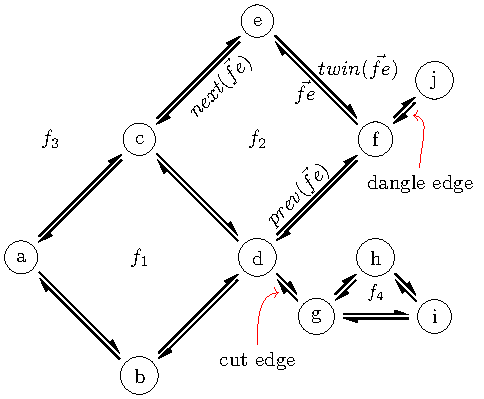
\includegraphics[width=0.6\linewidth]{chapterExtension/dcel_example2}
    \caption{Components of the DCEL structure with dangle and cut edges.}\label{fig:extension_dcel_example}
\end{figure}

In addition to the scalability issue, it is common in some applications that spatial polygons are provided in the form of scattered line segments, e.g., a set of road segments that form city blocks.  Such data can be very large and appear in applications in urban planning, geo-targeted advertising, economic and demographic studies, etc.  Yet, existing polygon overlay techniques cannot handle them directly at scale.  In that setting, extracting the DCEL subdivision's faces (polygons) is not straightforward.  To generate all of a subdivision's faces, the DCEL constructor must invoke a scalable \textit{polygonization} procedure, which extracts all closed polygons formed by a collection of planar line segments in a subdivision.

Furthermore, we extend the overlay method to support input polygons in scattered line segments form by integrating a scalable and distributed polygon extraction approach.  Our solutions have been implemented in a parallel framework (i.e., Apache Spark).

It should also consider the \textit{dangle} and \textit{cut edges} (see Figure  \ref{fig:extension_dcel_example}) resulting from the polygonization process and their intersection with other polygon layers.

This chapter extends the previous work in \cite{calderon_scalable_2023}. The main new contributions are summarized as follows. First, we introduce a new spatial partitioner, based on the kd-tree partitioning strategy, for constructing overlay  DCELs (section \ref{sec:kdtreestrategy}). Since it better utilizes the data  distributions in optimizing DCEL partitions, it leads to noticeably improved performance. The new partitioning strategy contrasts with the original strategy that employed space-partitioning techniques based on quadtrees. Second, we enable overlay DCELs to take scattered and noisy line segments as input instead of being limited to clean polygon data.  This builds on the work on scalable polygonization in \cite{abdelhafeez_ddcel_2023} to enable overlays of real datasets that consist of massive sets of line segments that cannot currently be handled by any existing technique. We also provide additional experiments, to quantify the benefits of the kd-tree based strategy, as well as the performance on the datasets with large volumes of line segments.

%\ref{sec:polygonization}
\textcolor{red}{Section XX} details the polygon extraction process for line input adaptation. It also extends the overlay method by supporting the overlay of dangle and cut edges.
